\chapter{Cuadricoptero con vision artificial}\label{sec: Cuadricoptero}
En el presente capítulo se pretende abordar el diseño y la implementación de un cuadricóptero con la capacidad para el seguimiento de un objeto, haciendo uso para ello de una FPGA como parte fundamental, y algunas otras herramientas que se expondrán a lo largo de esta sección. \newline

\section{Diseño}
En la figura se presenta un esquema con un alto nivel de abstracción en el que se da una primera aproximación del funcionamiento del sistema general.

\begin{figure}[H]
	\center
	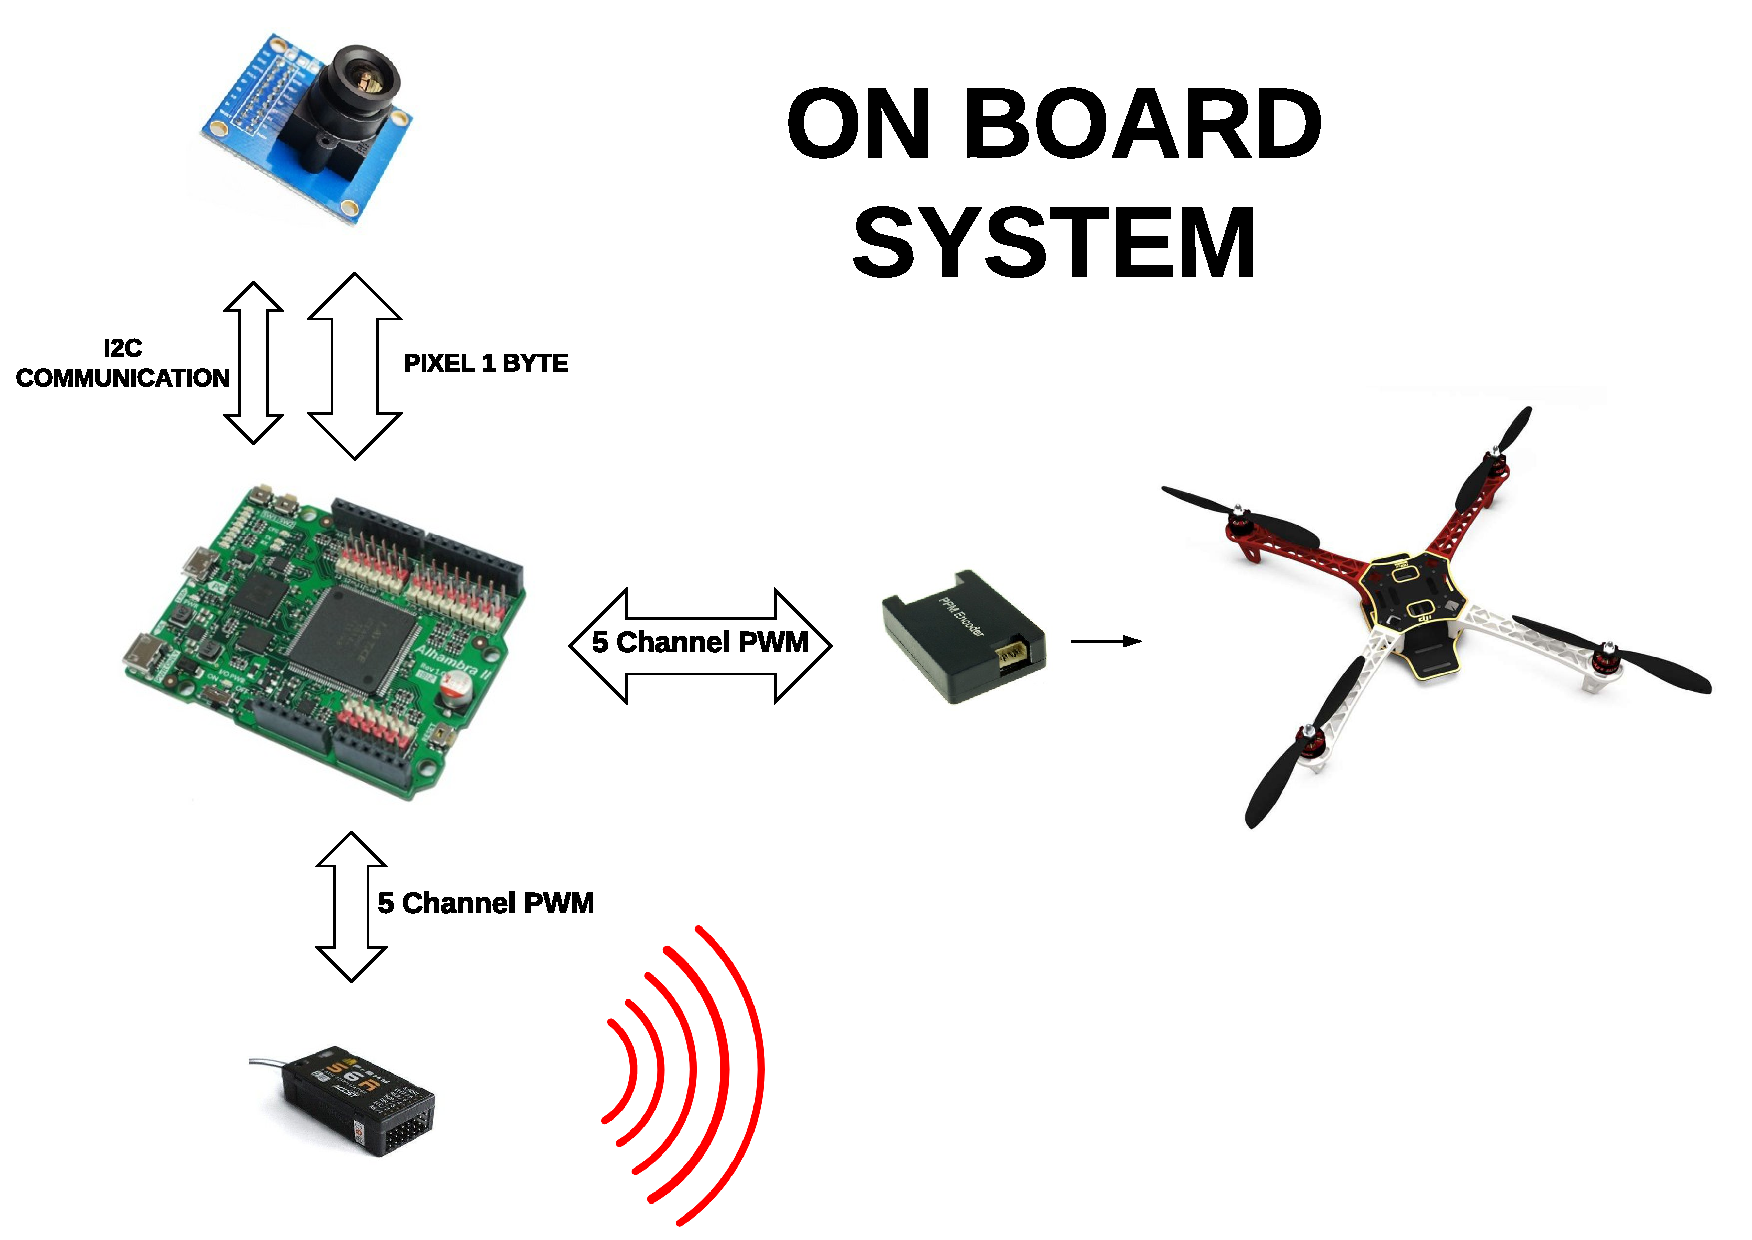
\includegraphics[trim = 0mm 0.5cm 0mm 0.5cm, clip,scale=0.4]{imagenes/Cuadricoptero_vision/on_board.pdf}
	\caption{Diseño a alto nivel del cuadricóptero con visión.}
	\label{fig:on_board}
\end{figure}

Se diferencia en este diseño la parte del control de la estabilización y la parte de percepción. 
En cuánto a la parte de la percepción, una cámara de bajo coste se conectará a la FPGA la cuál deberá implementar todo el algoritmo de reconocimiento del objeto. Previo a ello, y mediante protocolo i2c la cámara sera configurada de modo que facilite ese reconocimiento. Posteriormente y como salida de este algoritmo de reconocimiento la FPGA generará 4 canales PWM correspondientes al yaw, pitch, roll y altitud. Se hace uso de un PPM encoder, el cuál transforma estas 8 señales PWM en un canal PPM, entrada del sistema de estabilización del cuadricóptero "Pixhawk".

\section{Implementación de la percepción}
El módulo OV7670 [] cuenta con un sensor de imagen CMOS VGA OV7670, que permite trabajar a un máximo de 30 cuadros por segundos y una resolución de 640x480 píxeles. Es un sistema en chip (System on Chip, SoC) que es capaz de realizar procesamiento de imágenes, como: control de exposición, gamma, balance de blancos, saturación de color, control de tono. Estos parámetros se pueden configurar  mediante la interface SCCB (Bus de Control de Cámara Serial).

Algunas de las características más importantes se presentan a continuación, y las cuáles pueden ser obtenidas de su datasheet:

\begin{itemize}
	\item Voltaje de operación 3.3 VDC 
	\item Corriente Sleep 20 $\mu$A
	\item Transmisión de datos 8bits en paralelo 
	\item Interface de control estándar SCCB, compatible con I2C 
	\item Lente óptico de 1/6” 
	\item Ángulo de visión (FOV): $25^{\circ}$C
	\item Resolución 640x480 VGA 
	\item Sensibilidad 1.3V / (Lux-sec) 
	\item Ratio Señal-Ruido (SNR): 46 dB 
	\item Alta sensibilidad en ambientes de poca iluminación 
	\item Bajo voltaje, adecuado para aplicaciones portátiles 
\end{itemize}

Una imagen del módulo OV7670 se representa en la \ref{fig:OV7670}.

\begin{figure}[H]
	\center
	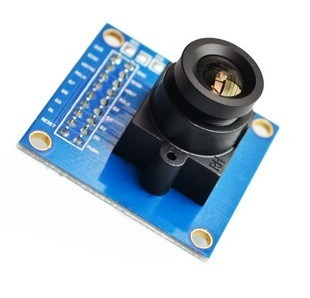
\includegraphics[scale=0.4, angle=0]{imagenes/Cuadricoptero_vision/OV7670}
	\caption{Cámara OV7670.}
	\label{fig:OV7670}
\end{figure}

La configuración de la cámara se realiza a través de una interfaz SCCB [], muy parecida a una comunicación I2C y cuyos registros se pueden encontrar en el datasheet. Por tanto, se ha de elegir una configuración adecuada para este propósito:

\begin{itemize}
	\item Se elije un tamaño de ventana de 640x480 debido a los pocos recursos de la tarjeta FPGA utilizada.
	\item El tipo de datos de salida será RGB, por la simplicidad en el uso. Obtendremos por tanto dos bytes por cada píxel capturado en el siguiente orden: 
	
		\begin{figure}[H]
			\center
			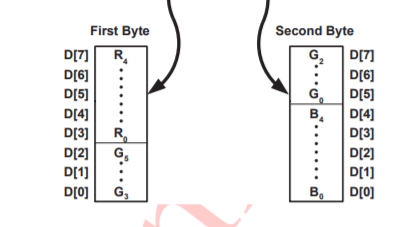
\includegraphics[trim = 0mm 0.5cm 0mm 0.5cm, clip,scale=0.6]{imagenes/Cuadricoptero_vision/pixel_OV7670}
			\caption{Formación de píxel en OV7670.}
			\label{fig:pixel_OV7670}
		\end{figure}
	
\end{itemize}

Para conseguir esa configuración es necesario una comunicación I2C con el módulo OV7670 que permite escribir en determinados registros.

El aspecto en IceStudio de esta escritura en I2C tiene el aspecto de la figura \ref{fig:I2C_write}.
\begin{figure}[H]
	\center
	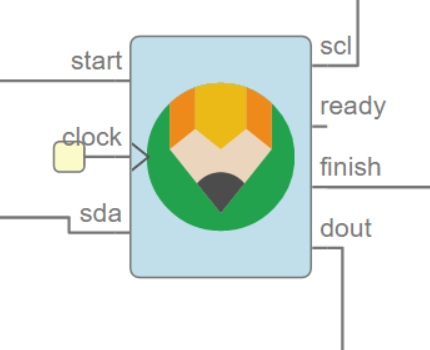
\includegraphics[scale=0.4, angle=0]{imagenes/Cuadricoptero_vision/I2C_write.PNG}
	\caption{Aspecto en IceStudio del módulo de escritura I2C.}
	\label{fig:I2C_write}
\end{figure}

Debido a que ha sido un módulo desarrollado íntegramente para esta aplicación, se representa el diagrama de flujo en la figura \ref{fig:i2c_write}

\begin{figure}[H]
	\center
	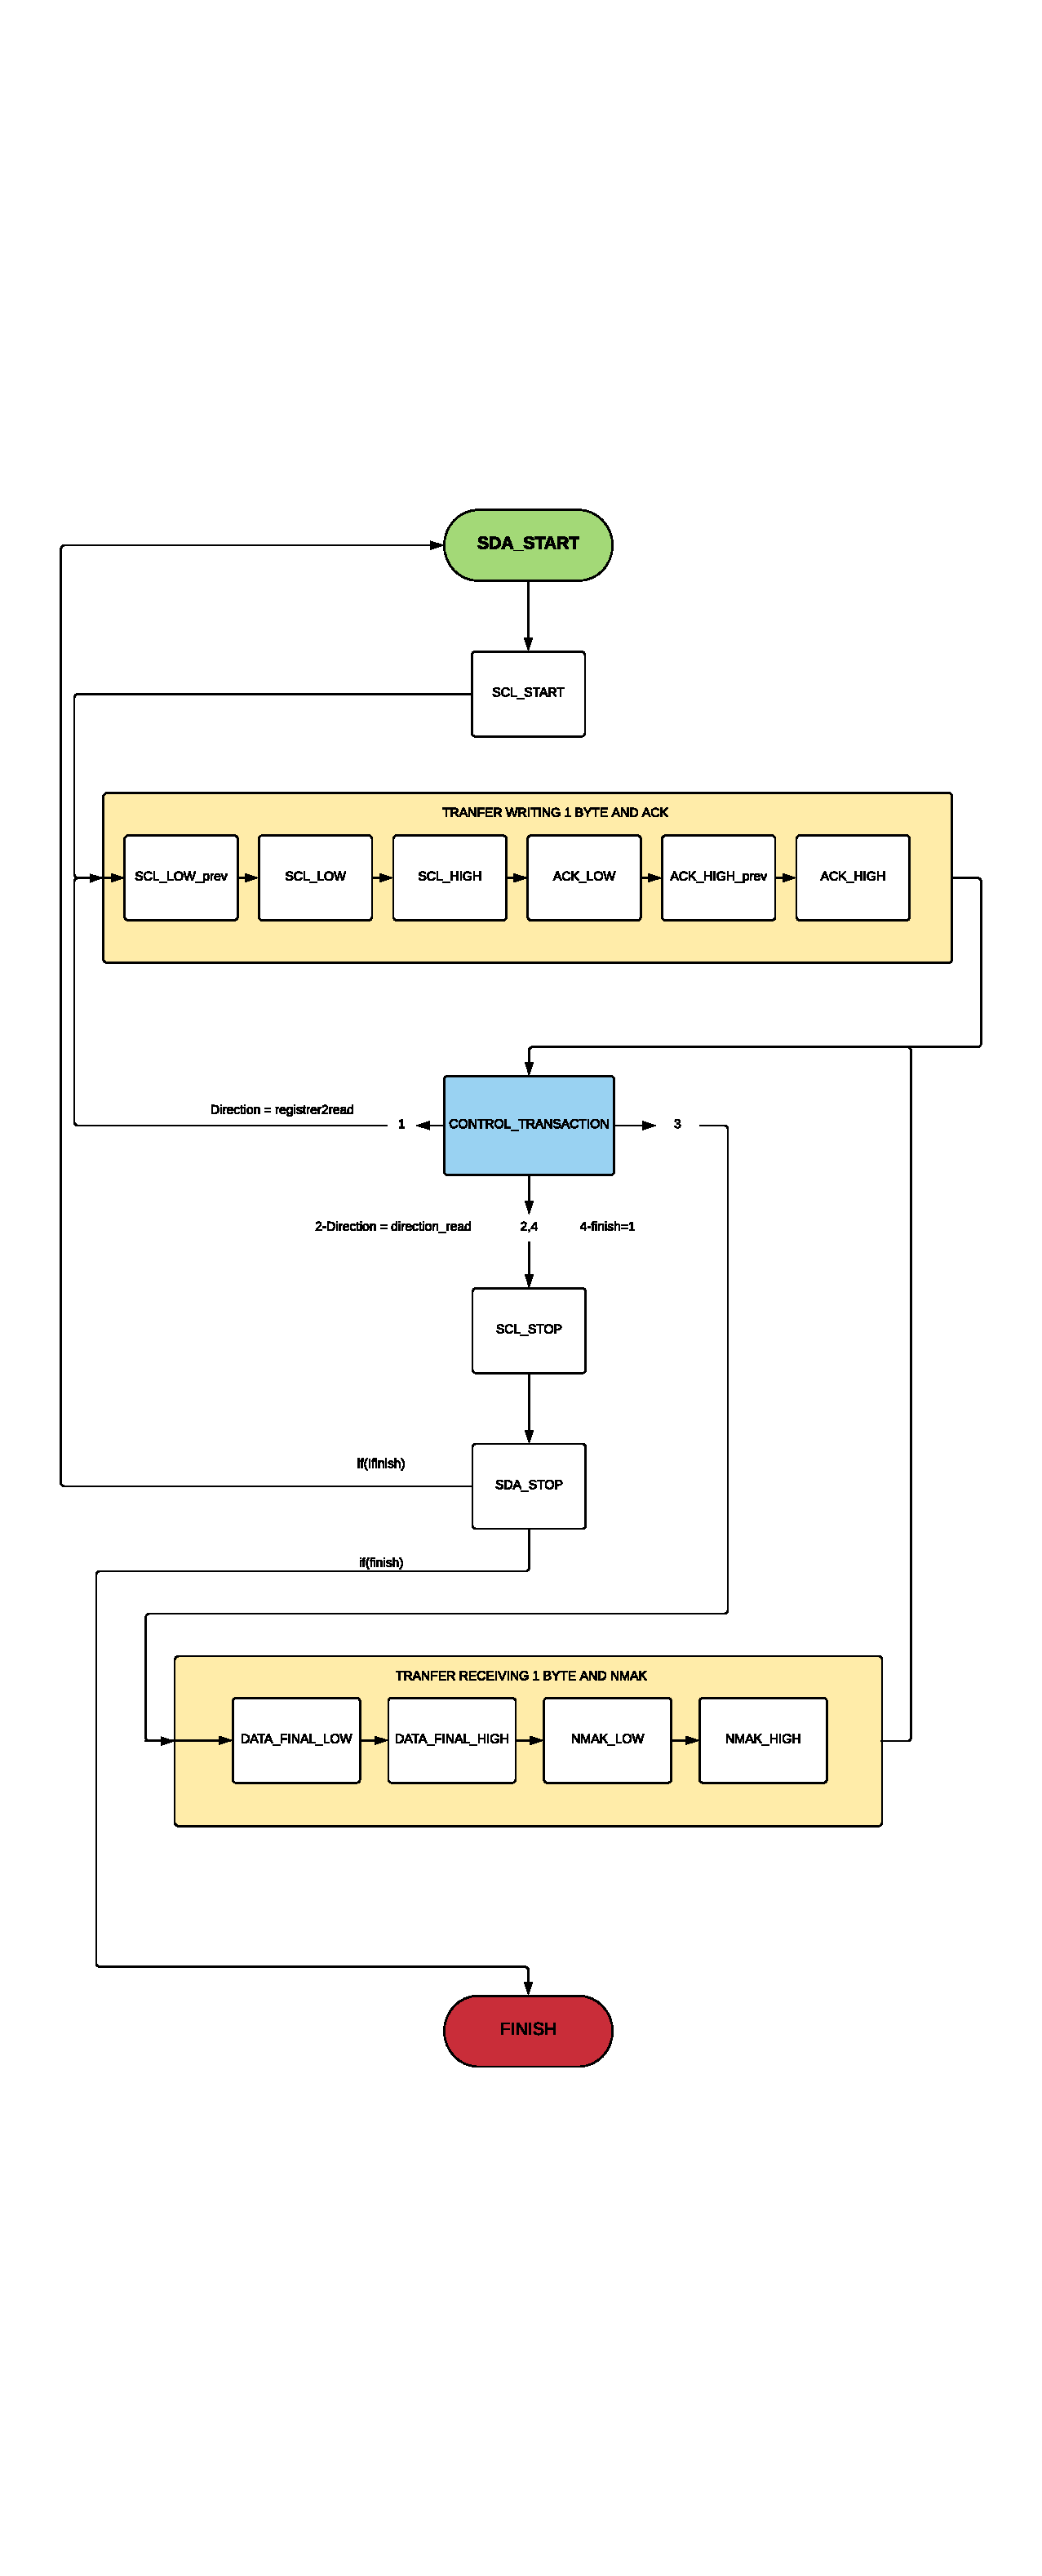
\includegraphics[trim = 0mm 6cm 0mm 6cm, clip,scale=0.5]{imagenes/Cuadricoptero_vision/I2C_WRITE.pdf}
	\caption{Diagrama de flujo de la escritura I2C.}
	\label{fig:i2c_write}
\end{figure}

Está compuesto por una máquina de 13 estados en los que cada uno tiene una función fundamental para conseguir el resultado deseado. Hay que trabajar a muy bajo nivel para evitar errores en la transmisión y dotar al sistema de las herramientas necesarias para la detección de posibles anomalías.

En una comunicación I2C es importante que tanto maestro como esclavo compartan los buses scl y sda, los cuáles estarán en alta siempre excepto cuando alguno de los dos anteriores impogan su paso a bajo nivel de voltaje, tierra en este caso. I2C basa su funcionamiento en reconocer en todo momento estos niveles de voltaje por lo que hay que asegurarse de que siempre exista la condición de que si el bus esta libre, el nivel de voltaje es alto. Para ello, ambos buses suelen tener una conexión a una resistencia de pull-up que facilite esta características y evite en todo momento posibles glitches de reloj, mala referencia de tierra, ruido, etc. El esquemático de conexiones de la camára será por tanto el representado en la \ref{fig:OV7670_schematic}.

\begin{figure}[H]
	\center
	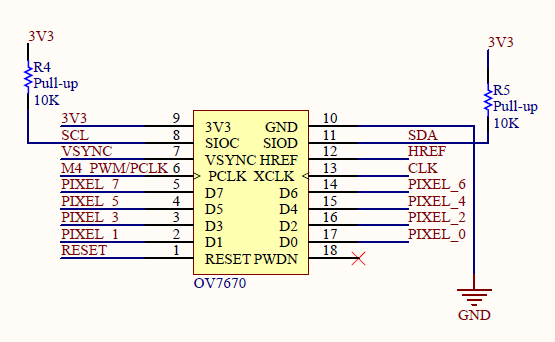
\includegraphics[scale=0.6, angle=0]{imagenes/Cuadricoptero_vision/OV7670_schematic}
	\caption{Esquemático para cámara OV7670.}
	\label{fig:OV7670_schematic}
\end{figure}

Uno de los problemas mas importantes en el desarrollo de este módulo recae el gobierno temporal de estos buses por parte del esclavo y el maestro. Para entenderlo se describe el ejemplo \ref{ejemplo:i2c}.

\begin{ejemplo}\label{ejemplo:i2c}
 Se requiere en primera instancia que el maestro imponga el bus SDA a alto nivel de voltaje.
 A continuación, el maestro debe quedarse a la espera de una contestación por parte del esclavo, el cuál es un dispositivo no controlado y externo a nuestro sistema. Cuando el esclavo intente escribir en el bus, se encontrará un nivel de voltaje impuesto por el maestro, y el cuál no se podrá cambiar.
\end{ejemplo}

Para corregir el problema expuesto en el ejemplo \ref{ejemplo:i2c} el dispositivo a la escucha deberá imponer un estado de alta impedancia eléctrica con respecto al bus. Se hace uso por tanto de un buffer triestado como el que se representa en la figura \ref{fig:buffer_triestado} y que permite ese comportamiento de manera controlada.
\begin{figure}[H]
	\center
	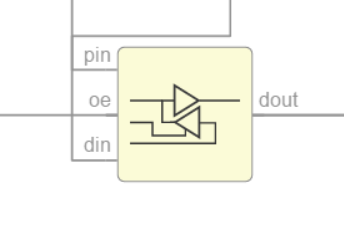
\includegraphics[scale=0.6, angle=0]{imagenes/Cuadricoptero_vision/triestado}
	\caption{Buffer triestado para bus I2C.}
	\label{fig:buffer_triestado}
\end{figure}

Un ejemplo de la escritura en I2C en el módulo OV7670 se representa en la figura \ref{fig:i2c_example}.

\begin{figure}[H]
	\center
	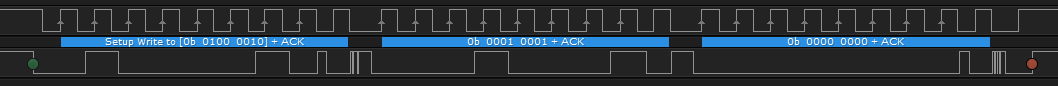
\includegraphics[scale=0.4, angle=0]{imagenes/Cuadricoptero_vision/i2c_example}
	\caption{Ejemplo de escritura I2C en OV7670.}
	\label{fig:i2c_example}
\end{figure}

\section{Implementación del control}
\section{Experimentos}









